\section{Tasarım, UML Diyagramları ve İş Planı}

\subsection{Kullanıcı Senaryoları ve Tipleri}
Bu bölüm altında kullanıcı senaryoları gösterilmiştir
\subsubsection{Yönetici Senaryoları}
\begin{figure}[h!]
    \centering
    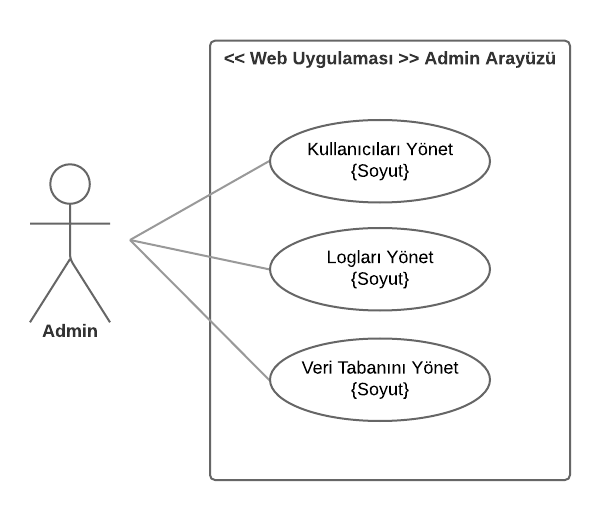
\includegraphics{Report/images/use1.png}
    \label{fig:use1}
\end{figure}
\newpage
\begin{figure}[h!]
    \centering
    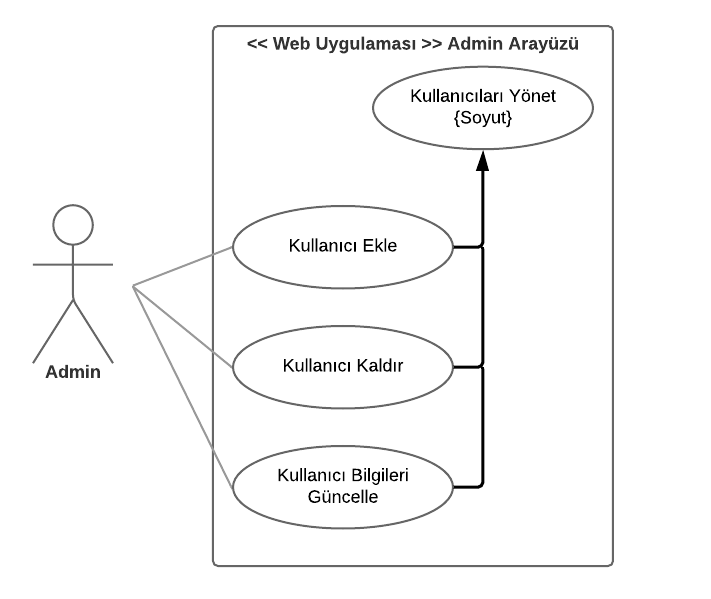
\includegraphics{Report/images/use2.png}
    \label{fig:use2}
\end{figure}
\newpage
\begin{figure}[h!]
    \centering
    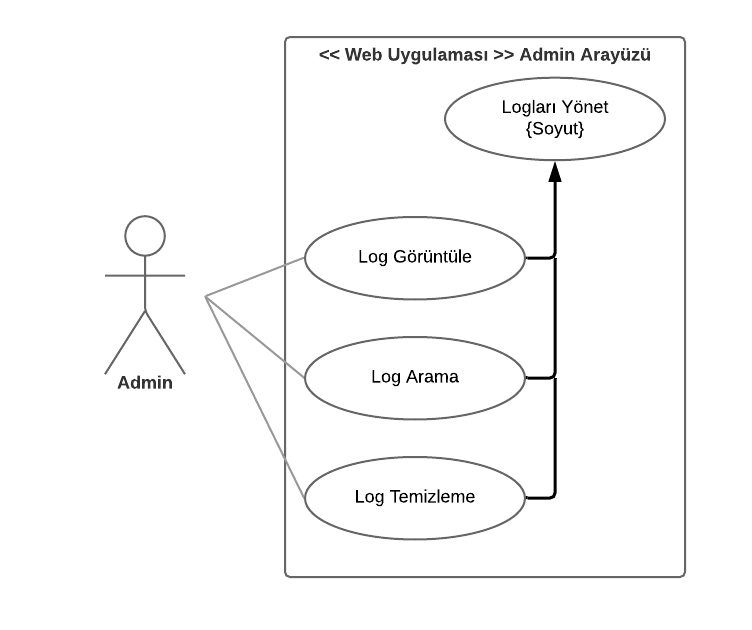
\includegraphics{Report/images/use3.png}
    \label{fig:use3}
\end{figure}
\newpage
\begin{figure}[h!]
    \centering
    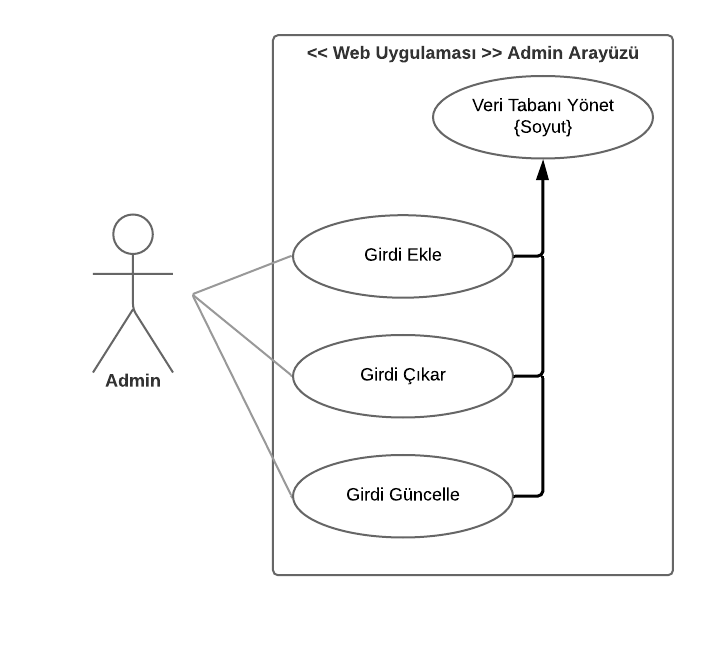
\includegraphics{Report/images/use4.png}
    \label{fig:use4}
\end{figure}
\newpage
\subsubsection{Normal Kullanıcı Senaryoları}
\begin{figure}[h!]
    \centering
    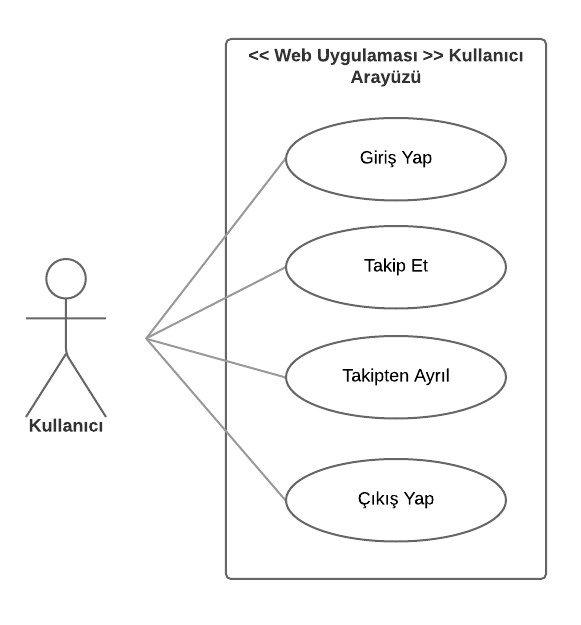
\includegraphics{Report/images/use5.png}
    \label{fig:use5}
\end{figure}
\newpage
\subsection{Sistem Mimarisi(High Level System Architecture)}
Bu bölüm altında yüksek level sistem mimari tasarımı gösterilmiştir
\begin{figure}[h!]
    \centering
    \includegraphics[width=\textwidth]{Report/sections/high-level.png}
    \label{fig:use5}
\end{figure}
\newpage
\subsection{İş Planı ve Modeli}
İş modeli olarak "Waterfall" modeli temel alınmıştır. İş planıda bu modele göre belirlenmiştir.
\begin{figure}[h!]
    \centering
    \includegraphics[width=\textwidth]{Report/sections/iş-planı.png}
    \label{fig:plan}
\end{figure}

\begin{itemize}
  \item 1. Adım ( 1. Ara buluşma kadar), Gereksinimler + Tasarım Basamağı
  \newline
Literatür araştırması, UML, use case ve high level system architecture diagram örneklerin incelenmesi ve proje için geliştirilip çizilmesi. Başarı kriterleri ve hedeflerin belirlenmesi.
  \item 2. Adım ( 2. Ara buluşmaya kadar), Gerçekleme Basamağı + Test Basamağı
  \newline
Kullanılacak diller ve frameworklerin kesinleştirilip araştılması ve öğrenilmesi.
  \item 3. Adım( 25 Kasım - 15 Aralık), Gerçekleme Basamağı + Test Basamağı
  \newline
Yazılım geliştirme döngüsü
  \item 4. Adım(15 Aralık - 26 Aralık), Son Eklemer Basamağı
  \newline
Çıktıların rapora eklenmesi, sunumların hazırlanması ve vidyo demo çekilmesi.
\end{itemize}

